\section*{Assignment 04: Monetisation Strategy}
\addcontentsline{toc}{section}{Assignment 04: Monetisation Strategy}

This section distils our spreadsheets into a monetisation plan that respects fragile network effects.

\subsection*{Revenue streams on the table}
\begin{itemize}
  \item \textbf{Completion fee on each project.} Organisations pay 7\% of the stipend once both sides mark the project successful, keeping monetisation tied to the value we orchestrate while staying invisible to students \citep{HagiuWright2013}.
  \item \textbf{Enablement subscription.} Larger NGOs and public agencies can upgrade to a 499~DKK/month Partner tier that unlocks templated briefs, analytics, and a dedicated coach, mirroring \citet{Choudary2016}'s push for producer tools. A contingency price sits ready if pilots push back.
  \item \textbf{Talent insights add-on.} When we have enough data we sell aggregated skill trends to universities and municipal innovation units, guarded by differential privacy and explicit consent so we do not trigger the surveillance trap \citet{Zuboff2019} warns about. Corporate sponsorships stay shelved until impact metrics prove we can add them without crowding out NGOs.
  \item \textbf{Grant-backed scholarships.} Social-impact grants subsidise student stipends for NGOs who cannot afford the fee so inclusion improves while subsidies still accelerate network effects \citep{ShapiroVarian1999}.
\end{itemize}

\subsection*{Timing across the platform lifecycle}
I anchor the roadmap in the classic seed $\rightarrow$ grow $\rightarrow$ harvest logic \citep{Choudary2016}.
\begin{enumerate}
  \item \textbf{Seeding (0--6 months).} No fees yet; we sign memoranda of understanding, chase 30 completed projects, and focus on trust rituals such as office hours and templated retrospectives.
  \item \textbf{Early growth (months 7--12).} Introduce the 7\% completion fee for new organisations while grandfathering the original cohort for three months, pilot the Partner tier with five agencies, and track completion above 85\%, churn below 10\%, and a net promoter score above +30.
  \item \textbf{Mature growth (beyond month 12).} Scale the fee to everyone, roll out the Partner tier broadly, launch the insights add-on, and track revenue per active organisation alongside NPS and tool adoption so monetisation deepens engagement.
\end{enumerate}

\subsection*{Experiments and guardrails}
To maintain analytical discipline, we run three experiments: an A/B test on when organisations see the completion fee, Van Westendorp pricing interviews to validate the Partner tier before hard-coding 499~DKK, and a 15-person diary study on whether insights reporting feels empowering or intrusive \citep{Reillier2017}. The A/B test compares disclosure at brief creation versus post-match; the pricing study clears the bar if the acceptable range averages 449--549~DKK; and the diary study keeps a rollback plan ready if trust drops below 70\%.

Cost mapping keeps us grounded: fixed year-one spend is 620,000~DKK for builders, design, and hosting, variable costs follow finished projects, and break-even lands near 1,050 projects per year, matching Assignment~09 and \citet{ShapiroVarian1999}.

Figure~\ref{fig:student-profile} puts a face on monetisation: the upgraded student profile surfaces badges, skill heatmaps, and endorsement timelines so NGOs can review talent quickly, while the ``next skill to showcase'' nudge keeps the data network effect tangible.

\begin{figure}[H]
  \centering
  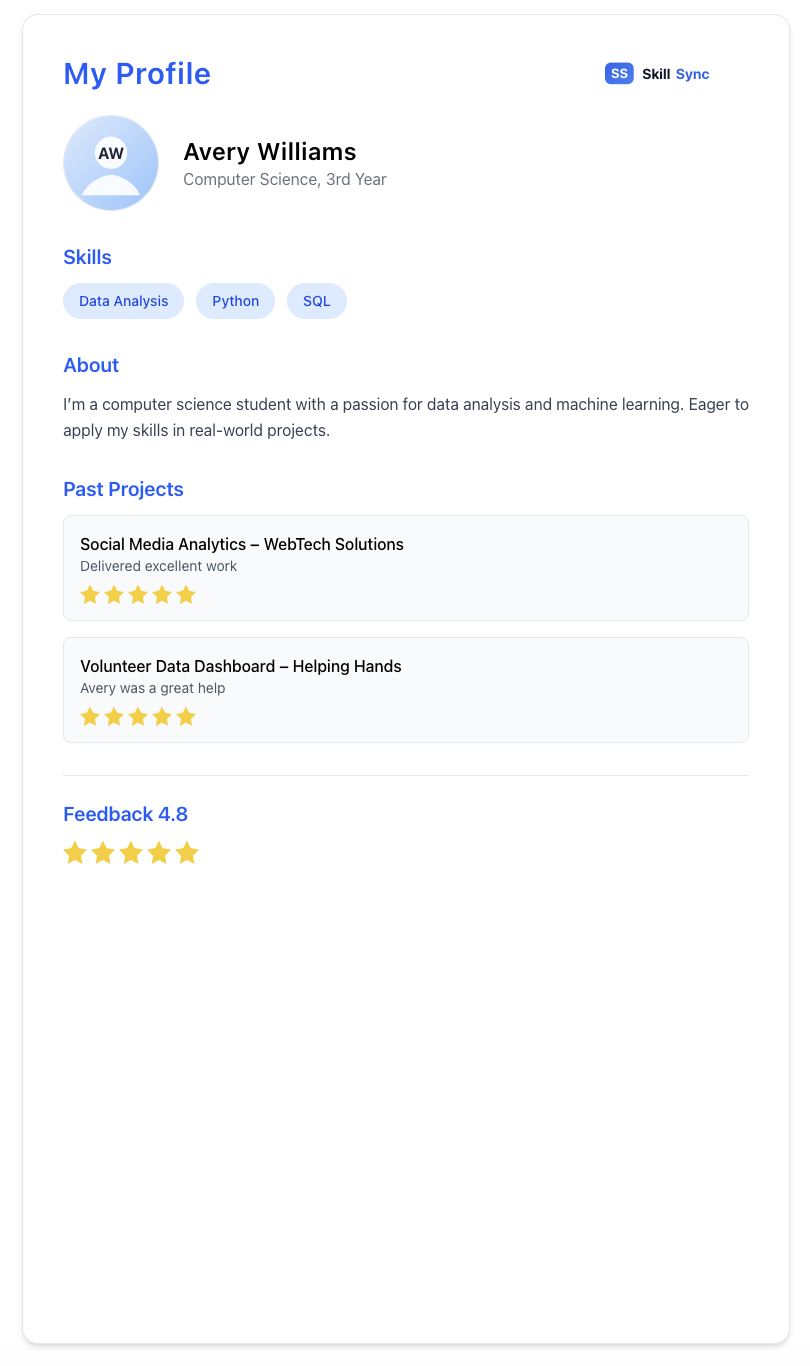
\includegraphics[width=0.8\linewidth]{Student-Profile.png}
  \caption{Student profile highlighting badges, heatmaps, and nudges.}
  \label{fig:student-profile}
\end{figure}

Figure~\ref{fig:student-profile} links richer profiles to faster NGO reviews.

Finally, we pressure-test ethical boundaries: the insights add-on ships only after five organisations in a sector and 500 projects, consent flows spell out ``why we collect this'' with easy opt-outs, and grants stay separate from transaction fees so subsidies never distort price signals \citep{Zuboff2019,Srnicek2017}.
